\section{CALM Analysis}

Bloom programs define unordered collections and rules that describe transformations over 
these collections.  A Bloom program may therefore be viewed as a dataflow graph with external 
inputs as sources, outputs as sinks and collections as internal nodes.  Given this view,
we may adapt powerful static analyses from the logic programming literature which are 
expresses as properties of the dataflow graphs.

In this section, we implement a simple key-value store in Bud, and analyze the implied
dataflow.  We begin with an interface for an abstract store, and evolve it first into a single-site
and finally into a replicated implementation.  Along the way, we use a dataflow visualization
to reason about the completeness and correctness of the supplied implementations.

\subsection{Predicate Dependency Graphs}

The Bud interpreter automatically generates a graphical
representation of dependencies between collections in a program
(Figures~\ref{fig:pdg-destructive-analysis} and \ref{fig:pdg-disorderly-analysis}).
Each node in the graph is either a collection or a cluster of collections; \textbf{table}s are shown as rectangles, ephemeral
collections (\textbf{scratch} and \textbf{channel}) are depicted as ovals, and clusters (described below) as octagons.  A
directed edge from node $A$ to node $B$ indicates that $B$ appears in the
lhs of a Bloom rule with $A$ referenced directly, or through a join expression,
in the rhs.  An edge is annotated based on the operator symbol in the rule and
the type of $B$.  If the rule is ``inductive''---i.e., has the \texttt{$<$+}
operator and a {\bf table} lhs---then the edge is marked with a $+$.  If the
rule is ``asynchronous''---i.e., a rule with the \texttt{$<$+} operator and a {\bf
channel} lhs---then the edge is a dashed line.  If the rule involves
non-monotonicity (aggregation or negation) over $A$, then the edge is marked with a $\lnot$.
%result in edges marked with a $\lnot$.
To make the visualizations more readable, any strongly connected component with both a $\lnot$ and a $+$ edge is collapsed into a octagonal ``temporal cluster,'' 
which can be viewed abstractly as a single, nonmonotonic node in the 
dataflow.\footnote{Datalog aficionados may be troubled by our mention of cycles
involving negation in the dependency graph.  In~\cite{dedalus} we
describe why the inclusion of a $+$ edge in such a cycle ensures stratifiability.}
%\jmh{capturing what? the fact that they must recurse over multiple timesteps? we can't just intro %this without any intuition.  You should also dismiss the particular collection names in this 
%figure as details from the KV store that are beyond the scope....}
%collapsing the mutually dependent collections into a single node.
Points of order are indicated in the graph by an edge with a white circle.
 Any negated edge in the graph is a point of order, as are all edges incident to a temporal cluster, including any self-edges.  Figure~\ref{fig:analysis-legend} provides a legend for the analysis visualizations.



\subsection{KVS Interface}

Figure~\ref{fig:kvs-proto} provides an abstract specification of a key-value store:
its interface to other Bloom programs or the external world.  
We may interact with any implementation of the store
by supplying inputs to \texttt{kvput} and \texttt{kvget} and by reading output from
\texttt{kvget\_response}.  
Much as we would expect to interact
with a hash table, we store key-value pairs by inserting them into \texttt{kvput}, and 
retrieve the value associated with a given key by inserting a tuple containing that key
into \texttt{kvget} and reading the result out of \texttt{kvget\_response}.  In each case,
we also require the caller to supply a unique request identifier \texttt{reqid} to differentiate
tuples in the event of multiple concurrent requests.
A module which uses a key-value store but is indifferent
to the specifics of the implementation may simply mix in this protocol specification
and postpone committing to a particular implementation until runtime.



\subsection{KVS Implementation}

Figure~\ref{fig:kvs-impl} completes the specification by supplying a very simple
realization of a key-value store.  Line~\ref{line:kvs-state} declares a \textbf{table}
called \texttt{bigtable} that stores the internal, persistent state of the store.
When a \texttt{kvput} tuple appears, its key-value pair is placed in \texttt{bigtable} in the
immediate next timestep(line~\ref{line:kvs-put}).  If a value for the given key already 
exists in \texttt{bigtable}, we wish to replace it with the newer value.  Line~\ref{line:kvs-join}
joins the input interface and internal state: if a row already exists for the current key,  
the join collection \texttt{jst} will contain a tuple that is the concatenation of the matching
tuples from \texttt{bigtable} and \texttt{kvput}.  In this event, line~\ref{line:kvs-clean}
states that in the immediate next timestep (and hence concurrently with the appearance of the
new tuple derived at line~\ref{line:kvs-put}), the old value associated with the given key
does not exist in \texttt{bigtable}.  


\subsection{Replicated KVS implementation}

Figure~\ref{fig:kvs-repl} extends the basic KVS module to support replication of the store
state.  It does so by mixing in MulticastProtocol, which provides the input interface 
\texttt{send\_mcast} and the output interface \texttt{mcast\_done}.  Line~\ref{line:rep-put}
declares an additional input interface (\texttt{kvput}) with the same name as the input
interface of the mixed in module BasicKVS.  This allows the writer of ReplicatedKVS to 
interpose additional logic between calls to KVSProtocol's input interface and the now 
``protected'' input interface of BasicKVS.  In ReplicatedKVS, references to \texttt{kvput}
appearing in the LHS of rules are resolved to the \texttt{kvput} provided by BasicKVS, 
while references in the RHS of rules resolve to the local \texttt{kvput}.
Note that this is unambiguous, because it is meaningless for a module to insert into its own input or to read data from its own output interfaces.

Thus, lines~\ref{line:send-mcast-beg}--\ref{line:send-mcast-end} ensure that when an external caller inserts a tuple into
\texttt{kvput}, its contents are marshalled (Line~\ref{line:marshall} into \texttt{send\_mcast}
if the originating address is not another replica (line~\ref{line:not-rep}).  The internal
\texttt{kvput} interface of BasicKVS is stimulated in one of two cases: if multicast succeeds
at the master replica (line~\ref{line:mcast-done}, or whenever a multicast is received at 
a peer replica (line~\ref{line:mcast-peer-beg}--\ref{line:mcast-peer-end}).

\subsection{Analyses}


Figure~\ref{fig:kvs-proto-pdg} presents a visual representation of the KVS protocol.  Data
flows from the source node (an external caller) to on or both of \texttt{kvput} and 
\texttt{kvget}, through some unknown dataflow, to \texttt{kvget\_response}.
The existence of the red diamond labeled ``??'' indicates that the dataflow is underspecified:
is must be ``completed'' by supplying dataflow that, at minimum, connects the input 
interfaces to the output interface.

Figure~\ref{fig:pdg-kvs-analysis} shows the visual analysis of the basic KVS implementation.




\begin{figure}[t]
\centering
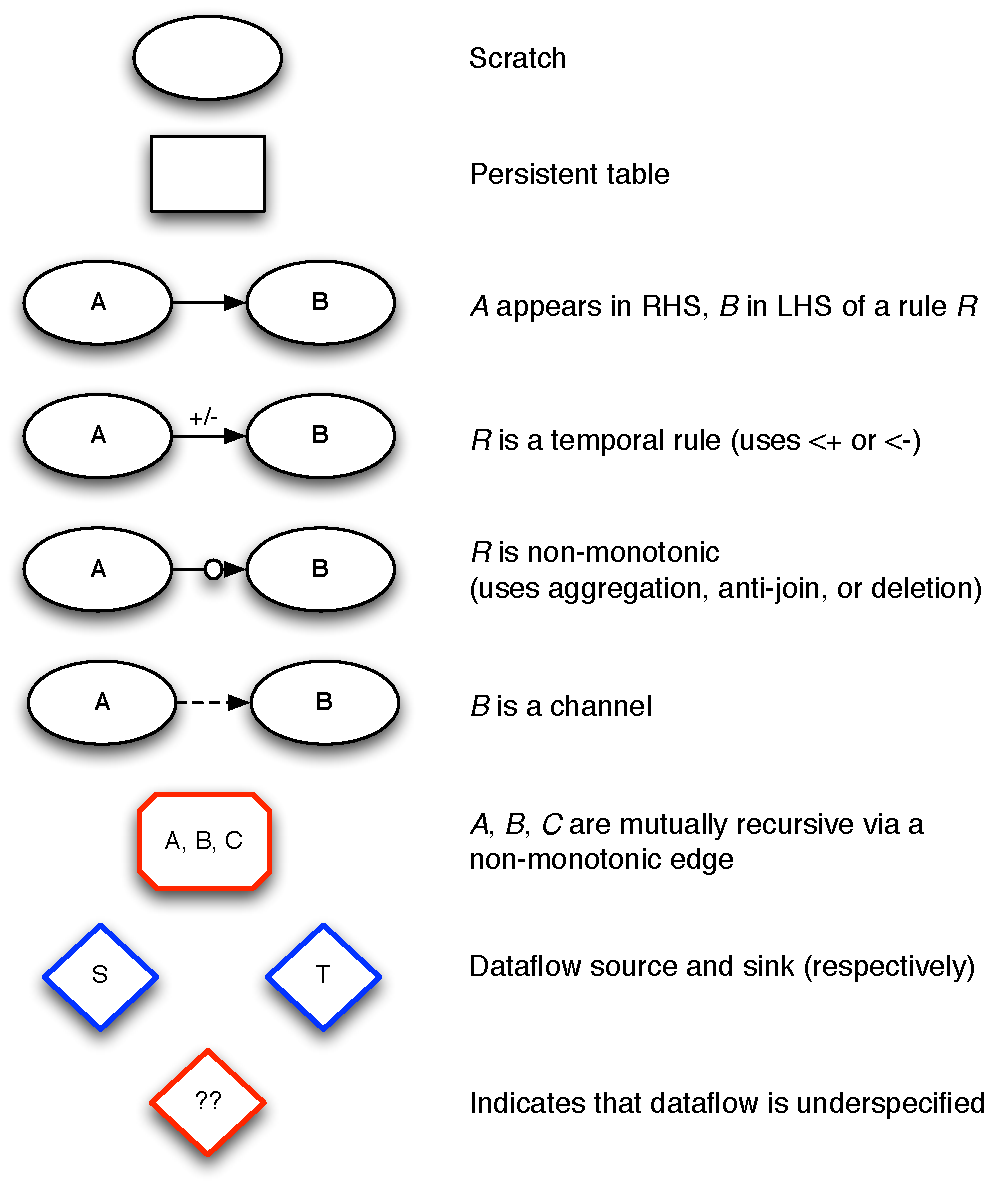
\includegraphics[width=1.1\linewidth]{fig/mittalk_legend.pdf}
\vspace{-10pt}
\caption{Visual analysis legend.}
\label{fig:analysis-legend}
\vspace{-2pt}
\end{figure}






\begin{figure}[t]
\begin{scriptsize}
\begin{lstlisting}
module KVSProtocol
  def state
    super
    interface input, :kvput, ['client', 'key', 'reqid'], ['value']
    interface input, :kvget, ['reqid'], ['key']
    interface output, :kvget_response, ['reqid'], ['key', 'value']
  end
end



\end{lstlisting}
\vspace{-10pt}
\caption{Key/value store protocol.}
\label{fig:kvs-proto}
\end{scriptsize}
\vspace{-2pt}
\end{figure}

\begin{figure}[t]
\centering
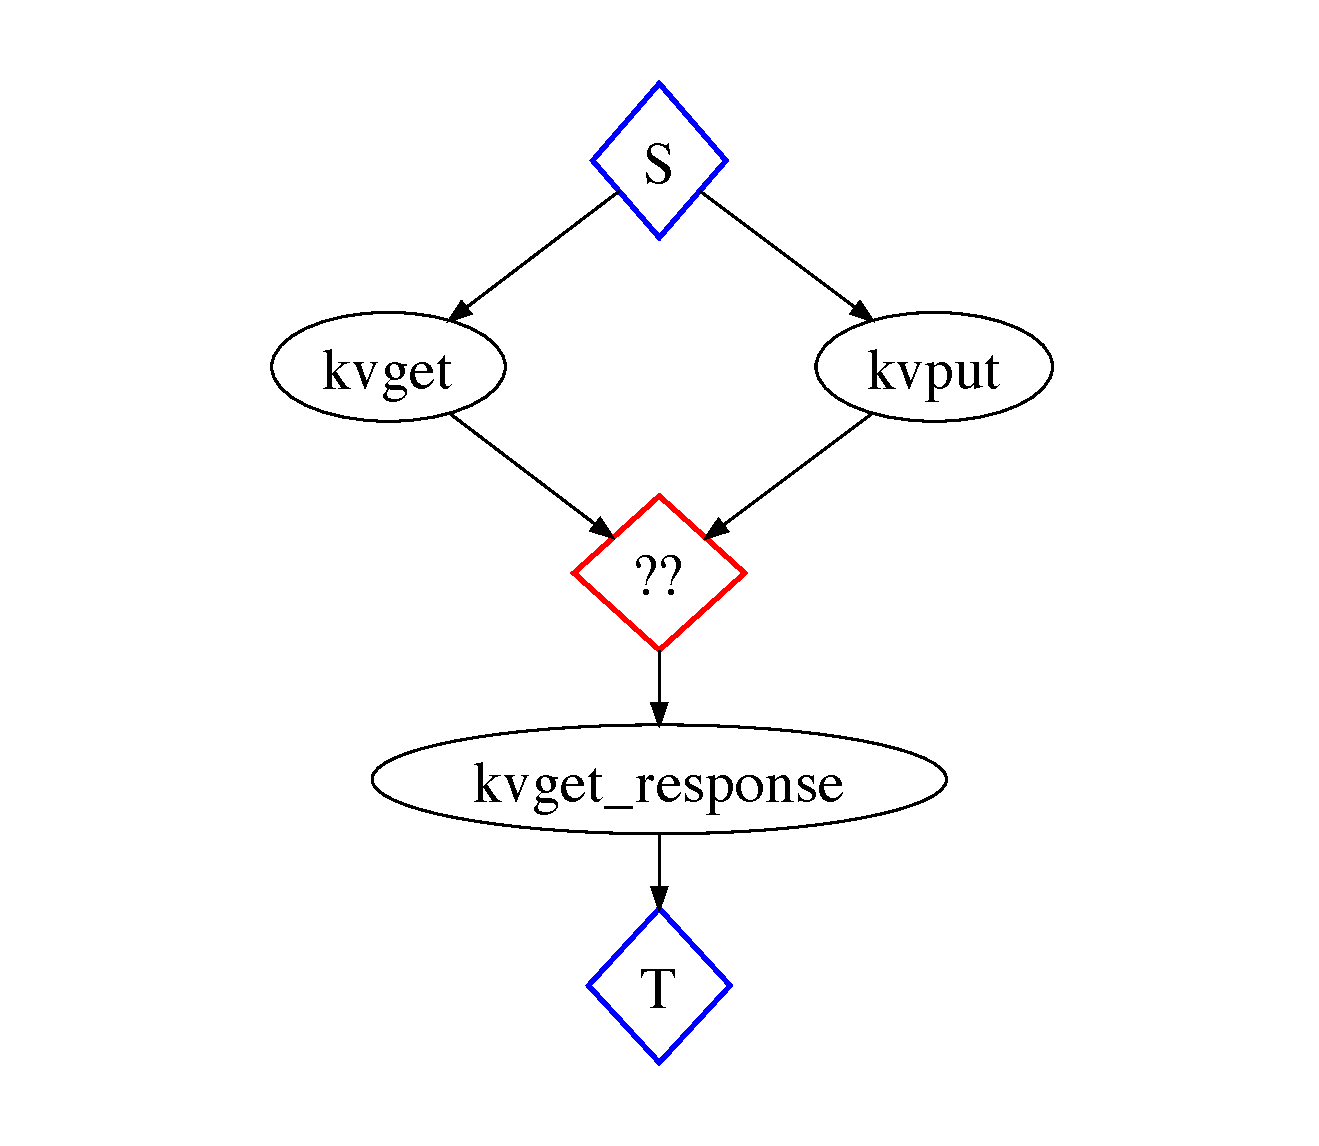
\includegraphics[width=0.4\linewidth]{fig/kvs_proto_pdg.pdf}
\vspace{-10pt}
\caption{Key-value store Protocol}
\label{fig:kvs-proto-pdg}
\vspace{-2pt}
\end{figure}


\begin{figure}[t]
\begin{scriptsize}
\begin{lstlisting}
module BasicKVS
  include KVSProtocol

  def state
    super
    table :bigtable, ['key'], ['value'] (*\label{line:kvs-state}*)
  end

  declare
  def mutate
    bigtable <+ kvput.map {|p| [p.key, p.value] } (*\label{line:kvs-put}*)
    jst = join [bigtable, kvput], [bigtable.key, kvput.key] (*\label{line:kvs-join}*)
    bigtable <- jst.map {|b, p| b } (*\label{line:kvs-clean}*)
  end

  declare
  def get
    getj = join [kvget, bigtable], [kvget.key, bigtable.key] (*\label{line:kvs-getjoin}*)
    kvget_response <= getj.map do |g, t|
      [g.reqid, t.key, t.value]
    end
  end
end


\end{lstlisting}
\vspace{-10pt}
\caption{Key/value store implementation.}
\label{fig:kvs-impl}
\end{scriptsize}
\vspace{-2pt}
\end{figure}


\begin{figure}[t]
\centering
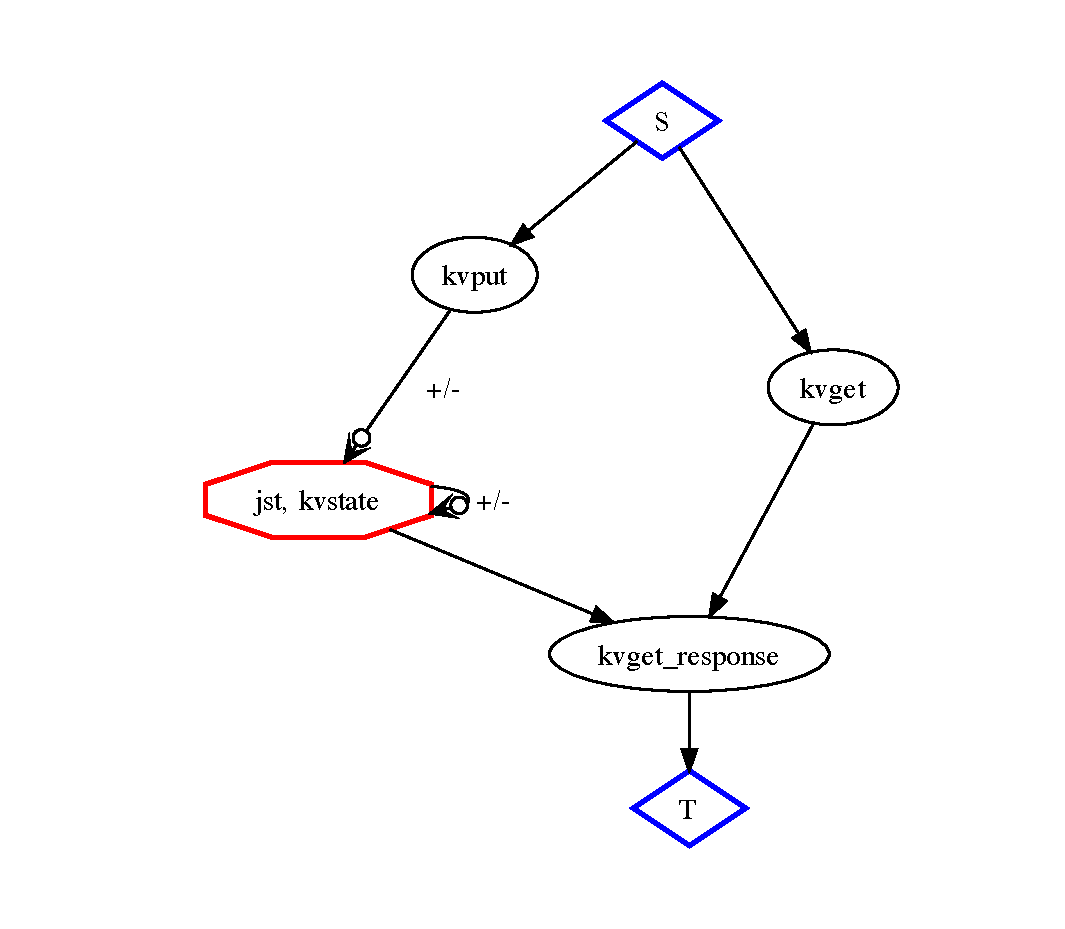
\includegraphics[width=0.5\linewidth]{fig/basickvs.pdf}
\vspace{-10pt}
\caption{Key/value store analysis.}
\label{fig:pdg-kvs-analysis}
\vspace{-2pt}
\end{figure}


\begin{figure}[t]
\begin{scriptsize}
\begin{lstlisting}
module ReplicatedKVS
  include BasicKVS
  include MulticastProtocol

  def state
    interface input, :kvput, ['client', 'key', 'reqid'], ['value']  (*\label{line:rep-put}*)
  end

  declare
  def local_indir
    send_mcast <= kvput.map do |k| (*\label{line:send-mcast-beg}*)
      unless members.include? [k.client]  (*\label{line:not-rep}*)
        [k.reqid, [@addy, k.key, k.reqid, k.value]]   (*\label{line:marshall}*)            
      end
    end (*\label{line:send-mcast-end}*)
    
    kvput <= mcast_done.map {|m| m.payload }  (*\label{line:mcast-done}*)

    kvput <= pipe_chan.map do |d| (*\label{line:mcast-peer-beg}*)
      if d.payload.fetch(1) != @addy
        d.payload
      end
    end (*\label{line:mcast-peer-end}*)
  end
end

\end{lstlisting}
\vspace{-10pt}
\caption{Replicated key/value store.}
\label{fig:kvs-repl}
\end{scriptsize}
\vspace{-2pt}
\end{figure}